

We search for robustness in the face of challenging scenarios. To this end we construct scenarios that represent two basic phenomena:
\begin{itemize}
    \item Moderate uncertainty at demand nodes, represented through addition of a random noise at the consumption site, e.g. associated with  response of gas-generators to renewable fluctuations on the electric-side of the system.
    \begin{equation}
        d_i(t) \to X_i(t)
    \end{equation}
    where
    \begin{equation}
        dX_i(t) = \alpha(d_i(t) - X_i(t)) + \gamma dW
    \end{equation}
    is a Ornstein–Uhlenbeck process - designed so that the mean is our nominal demand, $\mathbb{E}[X_i(t)] = d_i(t)$, and the variance approaches a constant exponentially fast:
    \begin{equation}
        \text{Var}(X_i(t)) = \frac{\gamma}{2\alpha}\left(1 - e^{2\alpha t} \right)
    \end{equation}
    The parameters were tuned heuristically to ensure $\alpha$ the mean was respected, and the variance approaches
    \begin{equation}
        \text{Var}(X_i(t)) \approx 0.01 \mu_i^2
    \end{equation}
    With $\mu_i$ being the mean withdrawal of node $i$. The noise for each demand is uncorrelated, a conservative approach which ignores geography and climate scales. Implementation on an actual system should be accompanied with data analysis and forecasts to determine realistic noise types for demands.
    \item Abrupt changes -- which we coin \emph{insults} -- that occur due to malfunction, weather or other exogenous circumstance. We focus particularly on supply challenges. That is, given a supply profile $s(t)$
    \begin{equation}
        s(t) \to s(t) + \Theta(t-T)\Gamma(t)
    \end{equation}
    where $\Theta$ is the Heaviside function, $T$ is the time of insult, and $\Gamma$ is the perturbation. For example, $\Gamma(t) = -s(t)$, simulates a complete loss of supply at time $T$.
\end{itemize}

In addition to studying bare ``do nothing'' scenarios we will also analyze mitigation by controls.  We assume that controls at the injection points (off-shore extraction sites at node \#1 and node \#8 in Fig.~\ref{fig:map}) and consumption sites, are step-wise. Operationally - due to the close coupling of Israel's gas extraction and delivery - step-wise control is preferable on the supply-side, while significantly idealized for demand nodes.

Focusing on the most challenging cases on fast ramps up (and, possibly, ramps down too) of consumption, e.g. around the time of sundown (or sunrise) in winter, we limit our analysis in this manuscript to \emph{prescribed} control. This allows us to conduct intuitive and easy to interpret tests of possible options. The goal of  this exploration is to analyze how the system operator can manage gas transients in line pack, meet power demand evolving throughout a day (or a number of days)  while also not exceeding the gas system pressure constraints. 

\begin{figure}
    \centering
    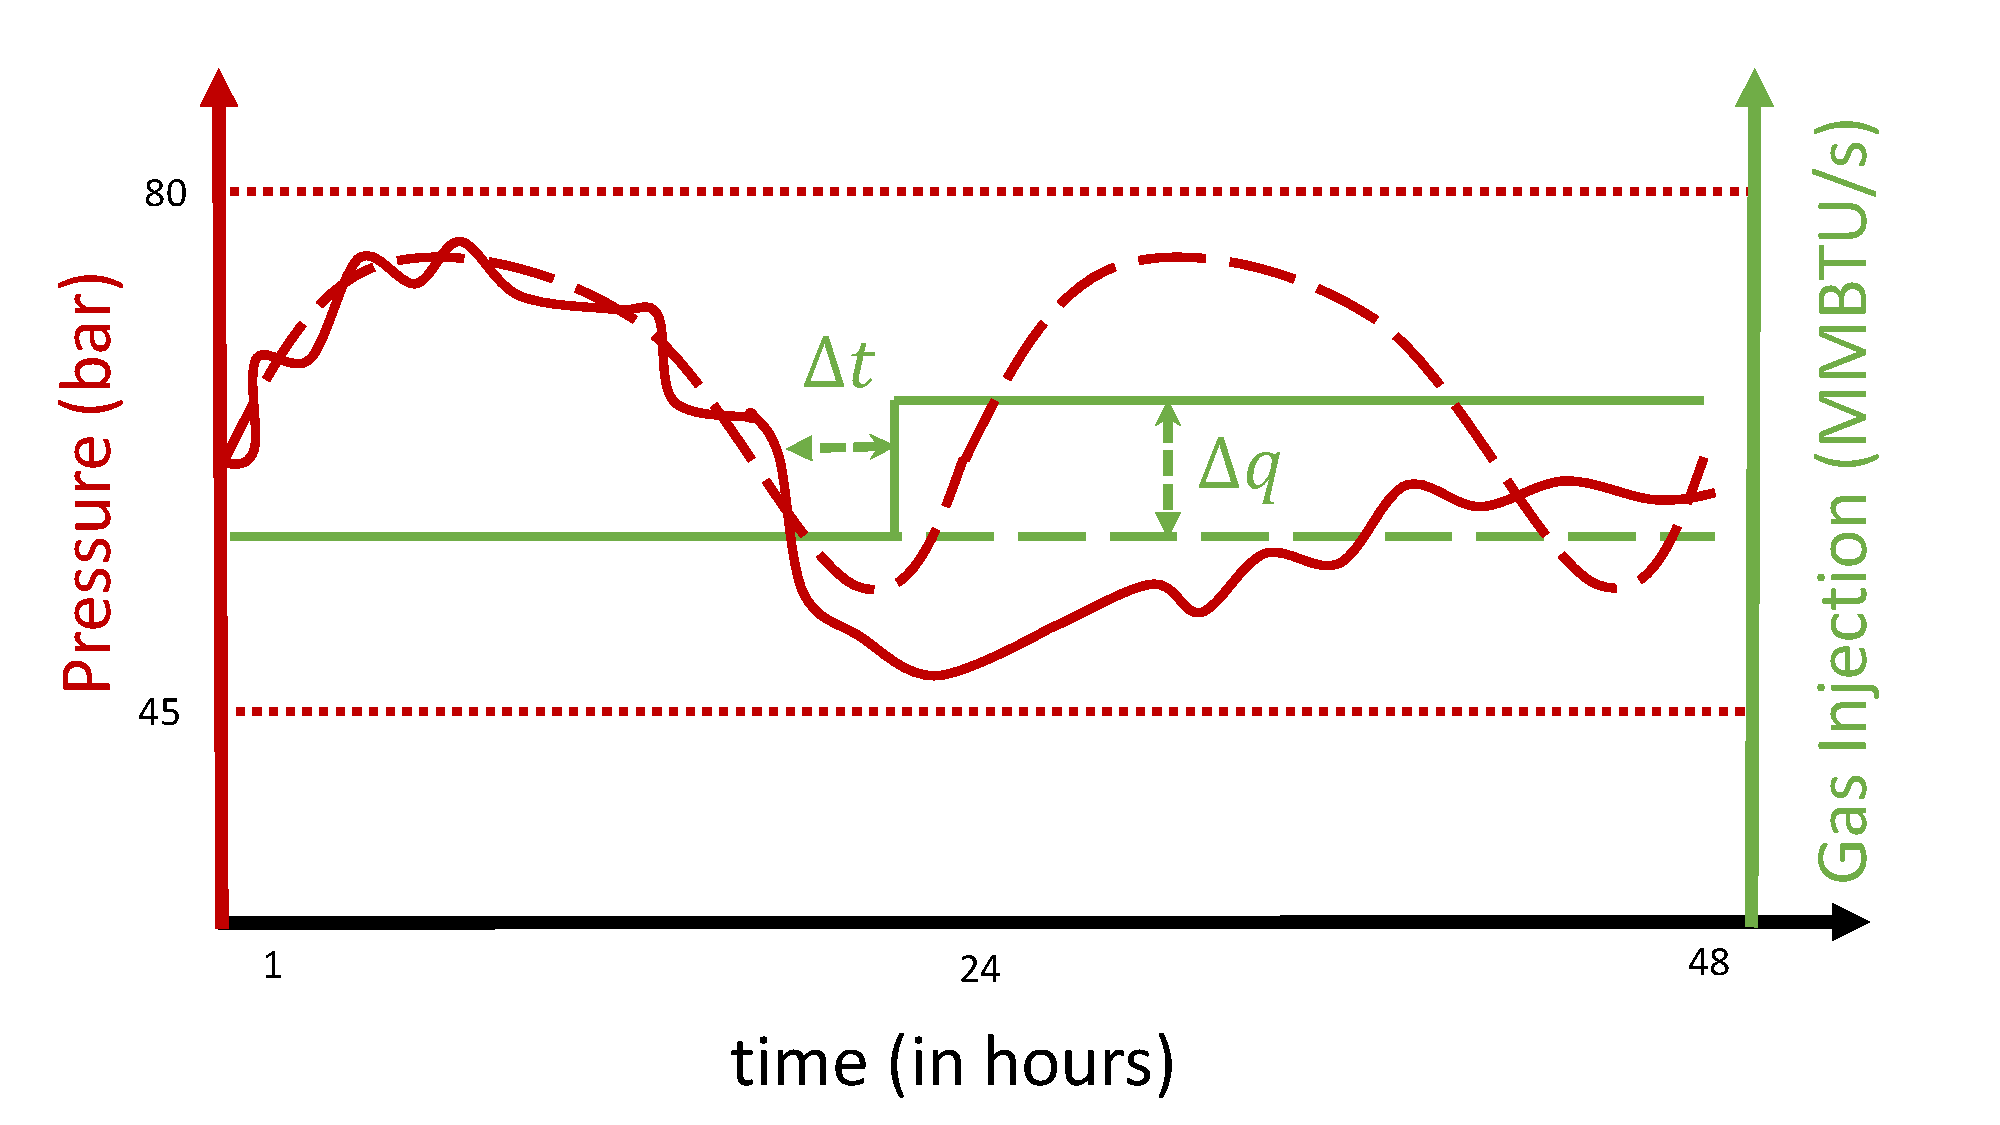
\includegraphics[width=0.4\textwidth]{figs/schematic.pdf}
    \caption{ Schematic illustration of the use cases of the system operations during an exemplary period of 48 hours. We show forecasts (long-dashed curves) and actual profiles (solid curves) for a pressure at a node and an injection at an entry point to the system,  where a control is applied in response to an insult. See text for details.
    \label{fig:schematic}}
\end{figure}

Our approach is illustrated schematically in Fig.~(\ref{fig:schematic}). Long-dashed green curve shows injection profile on one of the entry points to the system.  Typically,  it is flat where the value (in $MMBTU/s$) is computed based on the balanced forecast of consumption over the entire system and on the operational split of responsibilities between the injection points. Long-dashed red curve illustrates  forecast for a pressure at a node of the system.  Solid red curve shows an actual pressure profile,  which,  subject to typical uncertainty, largely follows the forecast till $\approx$ (hour) 23:00, when a significant insult occur and the deviation from the forecast becomes significant. Short-dashed red curves mark node-specific upper and lower limits for the pressure profile. Solid green curve shows operation profile at the injection point, which remains operational (in this use case) through out the 48 hours of observation, however the actual injection profile is not flat -- it follows forecast till hour $\approx$ 23:00+$\Delta t$ when a step-wise control action, responding to the $\approx$ 23:00 emergency, is applied. Selection of the proper time delay $\Delta t$, of the control response, and of the respective amplitude, $\Delta q$, constitutes a major operational challenge. 

% \begin{table}
% \begin{tabular}{|p{0.12\textwidth}|p{0.44\textwidth}|p{0.44\textwidth}|}
% \hline
% use case & description & emphasis \\ \hline\hline  
% sc.\#1 & nominal & variability\\ \hline
% sc.\#2-4 & insults at node \#1 of different types, no control &  survival time and location of the first pressure trouble vary \\ \hline
% sc.\#5-7 & insult as in sc. \#2, control at different (supply and export) nodes and of different types & survival time and location of the first pressure trouble vary\\
% \hline
% \end{tabular}
% \caption{Use cases.
% \label{table:use-cases}} 
% \end{table}


The approach to monitoring and prescribed control of the system is summarized in Table \ref{table:scenarios}. We present six scenarios of progressive stress. Each scenario is illustrated with a figure summarizing respective dynamics. (Animations of the pressure timeseries across the network, as well as software and data to reproduce all the results included here, can be found at \url{https://github.com/cmhyett/FluxControlLinepack}.)

We define a pressure crossing as when the nodal pressure falls below 50bar. The survival time $\tau$ is defined as the time between initiation of the insult and the time to first pressure crossing \textit{at any node}. 
Note that due to integrated random fluctuations of demand, we obtain distributions of survival times, shown for example in figure[\ref{fig:scen5}] as a shaded region about the median, annotated above with the node at which the pressure crossing occurred. To keep the picture clear, the figures only show pressure crossings for a subset of our nodes, namely 9,1, and 6, as they yield information regarding the north, middle and south of our network respectively. 

\begin{enumerate}
    \item Fig.~(\ref{fig:scen1}) shows pressures (dashed) and linepack (solid), in a flux-controlled, nominal week in August. It serves as our base case, and importantly, because of the constant flux at supply nodes, the temporal variation of pressure across the network is governed by the intra-day demand fluctuations.
\begin{figure}
    \centering
    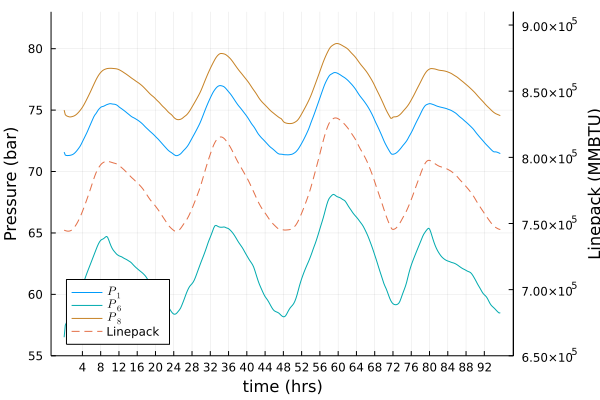
\includegraphics[width=0.47\textwidth]{figs/ScenarioResults/scen1.png}
    \caption{Nominal week in August, with no uncertainty.}
    \label{fig:scen1}
\end{figure}

    \item Fig.~(\ref{fig:scen2}) adds random fluctuations to demands on this nominal week - modeling uncertainty from exact power demand and generation of renewables. For each node, we add noise distributed uniformly with width of 5\% of nominal demand at that node. These small perturbations integrate over time, leading to significant linepack and pressure deviations from the mean.
    \begin{figure}
    \centering
    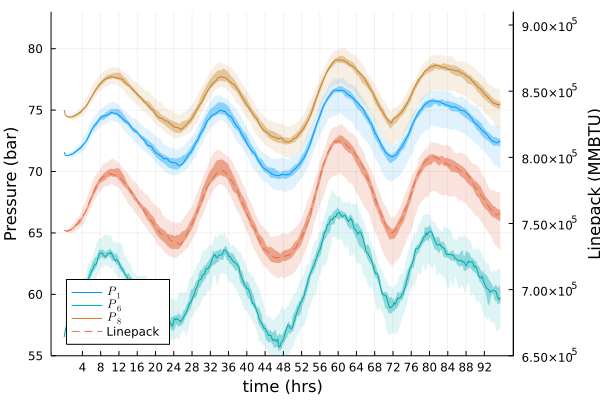
\includegraphics[width=0.47\textwidth]{figs/ScenarioResults/scen2.png}
    \caption{Nominal week in August, with empirical noise added to demand curves. Notice the drift of linepack and pressure jitter, consistent with what was predicted in \cite{chertkov_cascading_2014}. Using a Monte-Carlo with 50 simulations, we plot filled regions of containing the middle 75\%, 25\%, and median using increasing color intensities.}
    \label{fig:scen2}
\end{figure}

% \laurent{What is exact definition (e.g. with a formula) of an insult?}
    \item Fig.~(\ref{fig:scen3}) introduces an ``insult'' indicating off-nominal or emergency operation.  Particularly, supply at node \#1 (one of our two supply nodes) are closed at hour 36 in the simulation. We continue to run the simulation to observe the rate of linepack decay and the sequence of pressure crossings.
    The survival time in this scenario is
    \begin{equation}
        \tau = 4.13 \pm 0.38 \text{ hrs}
    \end{equation}
    where the $0.38$ is the standard deviation.
    This information can be translated to spatiotemporal ``vulnerability'' of the gas network.
\begin{figure}
    \centering
    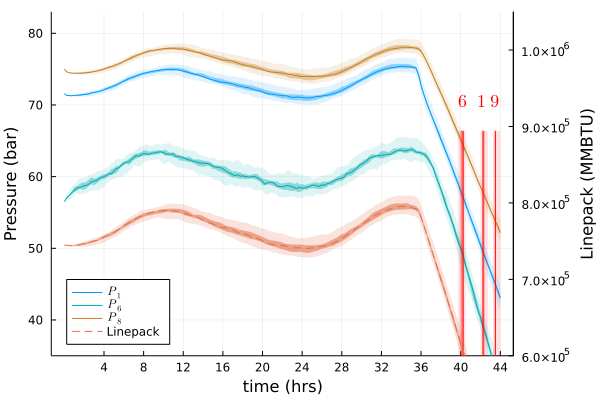
\includegraphics[width=0.47\textwidth]{figs/ScenarioResults/scen3.png}
    \caption{Scenario 3 results, an insult at a crest of the linepack at $t=36\text{hrs}$. Using a Monte-Carlo with 50 simulations, we plot filled regions containing the middle 75\%, 25\%, and median using increasing color intensities.}
    \label{fig:scen3}
\end{figure}

    \item Fig.~(\ref{fig:scen4}) introduces the same insult as scenario 3, but at hour 48 instead of hour 36. In particular, this corresponds to the insult occurring at a trough of the linepack curve instead of a peak. We highlight first that the time to first pressure crossing survival time is shorter in this case
    \begin{equation}
        \tau = 3.58 \pm 0.89 \text{ hrs}
    \end{equation}
    This simple statement that the survival time of the network depends on the start time of an insult is the result of complicated interactions between demand-node boundary conditions as well as network topology.
\begin{figure}
    \centering
    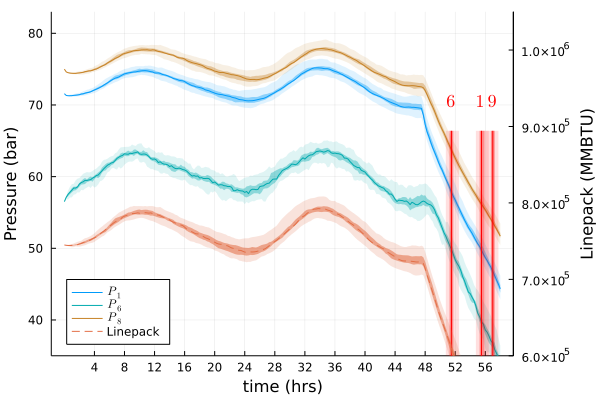
\includegraphics[width=0.47\textwidth]{figs/ScenarioResults/scen4.png}
    \caption{Scenario 4 results, an insult at a trough of the linepack at $t=48\text{hrs}$. Using a Monte-Carlo with 50 simulations, we plot filled regions containing the middle 75\%, 25\%, and median using increasing color intensities.}
    \label{fig:scen4}
\end{figure}

    \item Fig.~(\ref{fig:scen5}) begins introducing control, attempting to mimic "human in the loop" control of the network under the insult described in scenario 4. In this scenario, the operator at the remaining supply (node 8), increases to the max flow-rate a half hour after the insult begins ($t=48.5\text{hrs}$). This control stabilizes the linepack in the short-term, but fails to handle the daily ramp near hour 60. In particular, the south of the network, far from the remaining supply contains all of the pressure crossings.
    \begin{equation}
        \tau = 14.17 \pm 4.07 \text{ hrs}
    \end{equation}
\begin{figure}
    \centering
    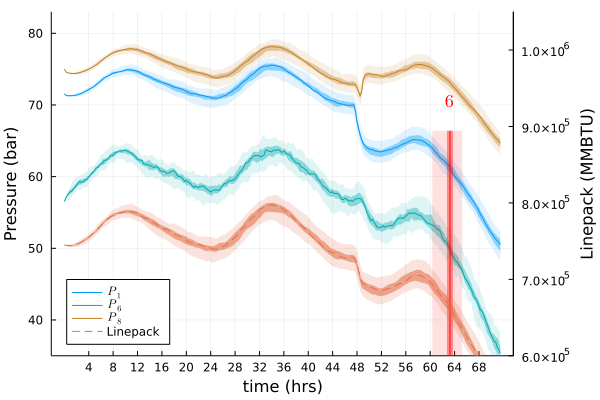
\includegraphics[width=0.47\textwidth]{figs/ScenarioResults/scen5.png}
    \caption{Scenario 5 results, introduces a step-wise increase in supply at node 8 half an hour after the insult ($t=48.5\text{hrs}$).}
    \label{fig:scen5}
\end{figure}

    \item Fig.~(\ref{fig:scen6}) finally builds upon scenario 5 to additionally curtail demand 2 hours after the insult ($t=50\text{hrs}$). This translates to a variety of potential action, from high penalty demand-response (as demonstrated during heat waves in California) to the transition of natural gas plants to alternative fuels, or the utilization of stored power. %\misha{Need to add references.}
    \begin{figure}
    \centering
    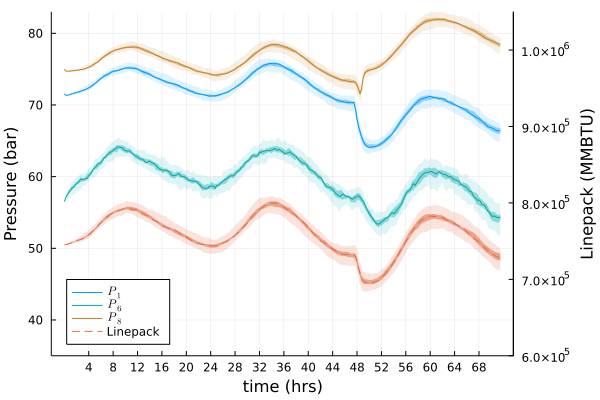
\includegraphics[width=0.47\textwidth]{figs/ScenarioResults/scen6.png}
    \caption{Scenario 6 results, curtails demand at $t=50\text{hrs}$, to maintain minimum pressures across the network.}
    \label{fig:scen6}
\end{figure}

\end{enumerate}

\begin{comment} 
\subsection{Illustrative Example}

For example, in the case of  the prescribed control at a supply node of the Israel gas system, modeled by  Eqs.~(\ref{eq:mass},\ref{eq:momentum}) extended to multiple pipes and accounting for injections/consumption at the nodes and for the fields continuity across the network, we pose the following question: if we can only control the supply via discrete jumps when should we introduce a perturbation (and of what magnitude) at the supply nodes to meet evolving (and also fluctuating demand), while keeping pressure relatively flat? In other words, we want to increase supply to match additional demand, with the objective to minimize the pressure deviations somewhere, e.g. at the supply, at the demand or, perhaps, somewhere in the middle. 

\misha{Criston, I suggest the following modification of the two schematic figures, Fig.~(\ref{fig:twoParametric}) and Fig.~(\ref{fig:minParamStudy_5node}). 

In the improved version of Fig.~(\ref{fig:twoParametric}) I suggest to show:
\begin{itemize}
    \item Pressure at a node of the network (left) vs adjustment of the injection/withdrawal at a control node. (Showing the case of flow control will make it a bit more clear --- will help to avoid confusion about two different pressures we need to discuss in the case when we have a pressure control. Having said this, we may want to mention after the illustrative example is shown that the pressure control is another option we will also consider in the manuscript.)
    \item For the pressure profile -- show (a) an evolving pressure forecast curve for the node, (b) an actual curve with a clear departure from the forecast, presumably associated with an insult, (c) corrected curve dependent on the timing and amplitude of the injection/withdrawal correction (may be good to show 2-3 options), (d) straight lines associated with upper and lower limits allowed at the node.
    \item For the  profile of injection/withdrawal at a node -- show (a) forecast curve for the control node injection/withdrawal, (b) the  (2-3) corrected option(s) equivalent to what we show for the pressure.
\end{itemize}
Wrt Fig.~(\ref{fig:minParamStudy_5node}). I am not sure we want to discuss the 5-node example in the paper. However, if we do, the 5 node example needs to be defined in words or shown in a figure. 
}

The schematics of the prescribed control is shown in Fig.~(\ref{fig:twoParametric}). Given a perturbation, e.g. perturbation of the withdrawal at the seconds of the abrupt (insult) type, we adjust (increase) supply changing it in a step-wise manner and probing different timing and amplitude of adjustment.  \misha{Add brief description, clear and preferably without formulas.} To illustrate, consider a $5$-node example shown in Fig.~?? \misha{Criston, please add figure showing the 5-node example.} 


denote step-wise control at a single supply node, $s$ , $c(t;x)$ at a single supply node $s$, and introduce our perturbation there. Further, let the boundary condition at $s$ be on pressure, and suppose that it is constant $p_s(t) = P$. Then, the control becomes, 
$c(t;x) = c_s(t) = dP\cdot \Theta(t-t_0)$, where $\Theta(x)$ is the Heaviside function and the
boundary condition is 
$$
    p_s(t) = 
        \begin{cases}
        P &\text{ if }t < t_0\\
        P + dP &\text{ if }t \geq t_0.
    \end{cases}
$$
Suppose now that the location in which we want to minimize variation is $x_0$. Changing $c(t;x)$ we seek to minimize the maximal value (over the network) between the perturbed and nominal values of the pressure. %mismatch between , $\min_{c(t;x)} \max |P_{perturbed}(t;x_0) - P_{nominal}(t;x_0)|$.
A simple approach to addressing this optimization question consists in looking for the point when the additional supply be felt at a demand node. In other words, we are asking what is the time delay between increasing the pressure at the supply and the pressure increasing at the demand? The setting is illustrated on a simple 5-node example in Fig.~(\ref{fig:twoParametric}). \misha{Criston, please add a one sentence description of the 5-node example.} 



\begin{figure}
    \centering
    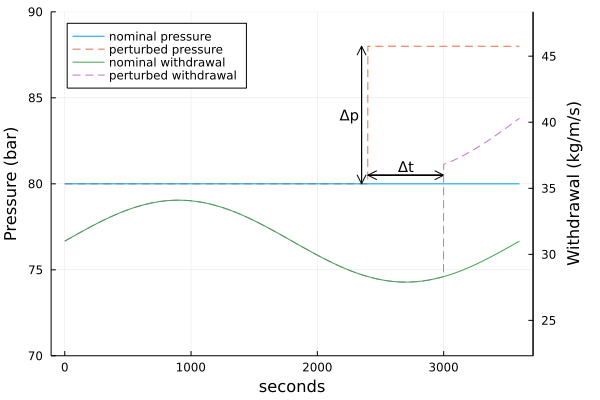
\includegraphics[width=\textwidth]{figs/twoParameterExample.png}
    \caption{Schematic of the prescribed control study %minimal parameter study 
    showing nominal and perturbed curves. The challenge will be to choose $\Delta p, \Delta t$ appropriately to minimize pressure variation in the system. 
    \label{fig:twoParametric}}
\end{figure}

In figure(\ref{fig:minParamStudy_5node}) we show results of the staggered-grid integration across the joint parameter space of $\Delta p, \Delta t$ control at node 1, to mitigate the effects of a sudden increase in consumption at node 4. These results suggest there is a characteristic time-delay between pressure increase at the supply node 1, and the consumption node. This timescale can be found by computing the minimal path length $\ell$, and dividing by the characteristic velocity $u_0 = \phi_0/\rho_0$, $\tau = \ell/u_0$.

\igal{In figure (1) bar is used for pressure, in figure (2) Pa is used, I think they should use same units. }  

\begin{figure}
    \begin{tabular}{cc}
        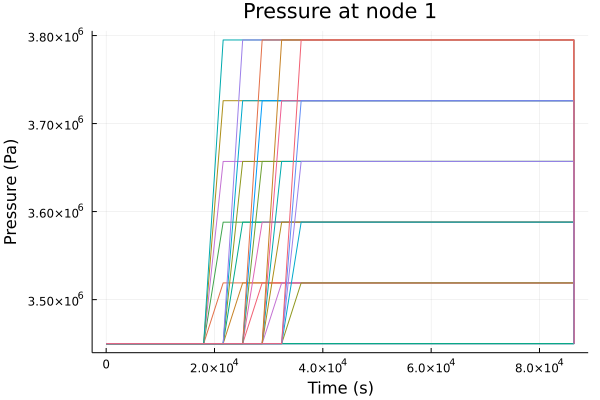
\includegraphics[width=0.5\textwidth]{figs/MinimalParameterStudy_5pipe/p1.png} &   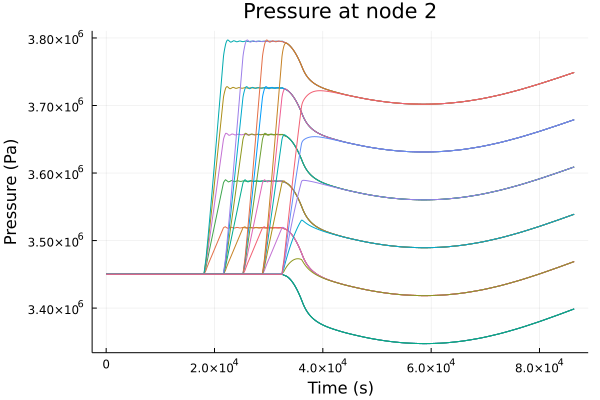
\includegraphics[width=0.5\textwidth]{figs/MinimalParameterStudy_5pipe/p2.png} \\
        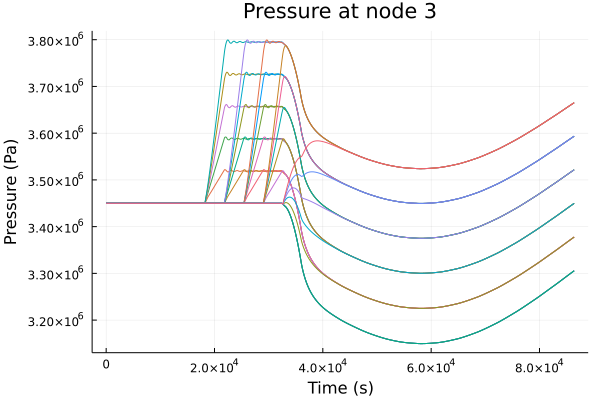
\includegraphics[width=0.5\textwidth]{figs/MinimalParameterStudy_5pipe/p3.png} &   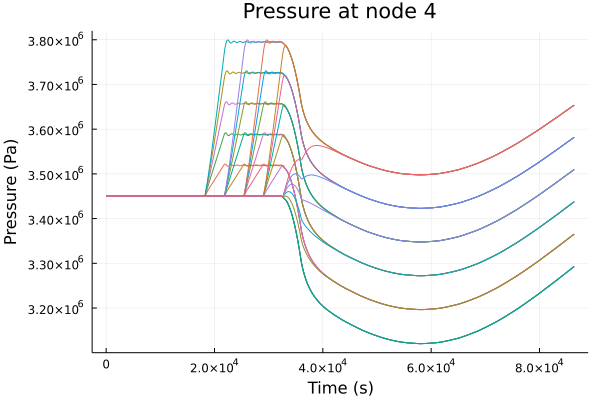
\includegraphics[width=0.5\textwidth]{figs/MinimalParameterStudy_5pipe/p4.png} \\
    \end{tabular}
    \label{fig:minParamStudy_5node}
\end{figure}
\end{comment}

